\documentclass[conference]{IEEEtran}
    \IEEEoverridecommandlockouts
    \usepackage{cite}
    \usepackage{amsmath,amssymb,amsfonts}
    \usepackage{algorithmic}
    \usepackage{graphicx}
    \usepackage{comment}
    \usepackage{balance}
    \usepackage{textcomp}
    \usepackage{xcolor}
    \usepackage{booktabs}
    \usepackage{amssymb}   % for \checkmark
    \usepackage{colortbl}  % coloured table cells
    \usepackage{pifont}    % \ding{55} cross mark
    \usepackage{tikz}
    \usepackage{pgfplots}
    \pgfplotsset{compat=1.18}
    
    \usetikzlibrary{shapes.geometric, arrows.meta, positioning, fit}
    \def\BibTeX{{\rm B\kern-.05em{\sc i\kern-.025em b}\kern-.08em
        T\kern-.1667em\lower.7ex\hbox{E}\kern-.125emX}}

    % ── TikZ styles ───────────────────────────────────────────────
    \tikzstyle{startstop} = [rectangle, rounded corners, minimum width=2.2cm,
        minimum height=0.7cm, text centered, draw=black, fill=red!20,
        font=\scriptsize]
    \tikzstyle{process} = [rectangle, minimum width=2.2cm, minimum height=0.7cm,
        text centered, draw=black, fill=blue!10, font=\scriptsize]
    \tikzstyle{decision} = [diamond, minimum width=1.8cm, minimum height=0.6cm,
        text centered, draw=black, fill=green!10, font=\scriptsize, aspect=2.5]
    \tikzstyle{io} = [trapezium, trapezium left angle=70, trapezium right angle=110,
        minimum width=2cm, minimum height=0.7cm, text centered, draw=black,
        fill=orange!15, font=\scriptsize]
    \tikzstyle{arrow} = [thick, ->, >=Stealth]

    \begin{document}

    \title{A Low-Cost Conductive Grid System for Real-Time\\
    Multi-Metric Braille Reading Performance Analysis}



    \maketitle

    % ---------------------------------------------------------------
    \begin{abstract}
    Objective assessment of Braille reading proficiency remains essential
    yet underserved, with existing tools either prohibitively expensive or
    unsuitable for widespread classroom deployment. This paper presents a
    scalable, low-cost conductive grid-based sensing system that detects
    multi-touch interactions over a $7\times7$ Braille sensing grid in
    real time. An ESP32 microcontroller drives a multiplexed row-column
    scanning architecture, streaming capacitively coupled touch frames to
    a host system over USB-serial. A multi-threaded Python pipeline
    computes seven complementary performance metrics: rolling Words per
    Minute (WPM) with exponential moving average smoothing, velocity
    profile inter-quartile range (IQR) as a motor-consistency indicator,
    inter-word regression rate and hesitation analysis, word-level
    Time-on-Task (ToT), grid coverage and skip-rate analysis, path
    efficiency with LOWESS trend fitting, and a composite difficulty score
    that unifies all signals into a per-word indicator. The system
    operates without any wearable device or optical apparatus, providing
    an unobtrusive, low-cost platform for diagnosing Braille reading
    proficiency in classroom and research settings.
    \end{abstract}

    \begin{IEEEkeywords}
    Braille reading, conductive grid, touch sensing, capacitive coupling,
    ESP32, finger tracking, WPM, time-on-task, regression analysis, path
    efficiency, motor consistency, accessibility, low-cost assistive
    technology
    \end{IEEEkeywords}

    % ---------------------------------------------------------------
    \section{Introduction}
    \label{sec:intro}

    Braille literacy remains a cornerstone of independence and academic
    achievement for individuals who are blind or visually impaired.
    Research consistently demonstrates that Braille-literate individuals
    enjoy substantially higher employment rates~\cite{b10}; however, the National Federation of the Blind reports a severe literacy crisis wherein nearly 90\% of blind children are not being taught to read and write Braille~\cite{nfb2009}. The World Health
    Organization further reports that vision impairment carries an annual
    global productivity loss of approximately
    US\$\,411 billion~\cite{b11}, underscoring the economic imperative of
    effective tactile literacy programmes. Yet despite this importance,
    tools for \emph{objectively} measuring and improving Braille reading
    skills remain scarce, expensive, and inaccessible to most educators
    and learners. Martiniello and Wittich~\cite{martiniello2022} confirm in a
    comprehensive scoping review that Braille reading performance is determined
    by at least three independent capacity dimensions including tactile sensitivity,
    manual dexterity, and cognitive processing, underscoring why aggregate WPM
    alone is insufficient for diagnostic assessment. A systematic review of
    technology-supported Braille literacy education for
    children~\cite{techbraillesysrev2022} further confirms that while electronic
    tools support Braille output, real-time performance monitoring systems remain
    absent from classroom practice, a gap the proposed platform directly
    addresses.

    Knowlton and Wetzel~\cite{b12} reported a mean Braille reading speed
    of 136 words per minute (WPM) for experienced readers in controlled
    reading tasks, with a range of 65--185\,WPM. While some literature claims that highly proficient readers can achieve rates between 200 and 400\,WPM~\cite{legge1999}, reflecting the upper tail of expert performance, beginners typically read at only 50-70\,WPM. Understanding \emph{why} a reader is slow, whether due
    to uneven finger movement, frequent backtracking, or inefficient
    reading patterns requires instrumentation that captures more than
    aggregate reading speed. Existing systems for analyzing Braille
    reading  rely on vision-based tracking, wearable sensors~\cite{divyansh-vlsid, divyansh-iccae, chinmay-sensors}, or
    dedicated electronic displays, all of which are intrusive, expensive,
    or impractical for widespread deployment.

    While low-cost real-time tactile tracking has been successfully demonstrated in other contexts such as interactive museum exhibits~\cite{ajay-tactile1, ajay-tactile2}, there is a pressing need to adapt such non-invasive approaches to capture continuous Braille reading interaction data. This includes tracking finger movement patterns, per-cell reading durations, total reading time, and average reading rate without instrumenting the reader.
    This paper presents such a system. A passive conductive grid placed
    beneath a $7\times7$ Braille sensing grid detects finger contact
    events through capacitive coupling; a multi-threaded software pipeline
    then computes seven complementary metrics that together profile both
    reading fluency and motor consistency. The key contributions of this
    work are:

    \begin{itemize}
        \item A low-cost, non-invasive conductive grid system capable of
            localizing touch interactions on a physical Braille page in
            real time.

        \item 
        A comprehensive multi-metric analysis of Braille reading performance by quantifying reading fluency, finger-motion stability, regressions and hesitations, time-on-task behavior, reading coverage, path efficiency, and overall word-level difficulty.
        
        %\item A real-time reading speed %estimation framework (WPM) for
            %monitoring Braille reading fluency.

        %\item A movement-consistency analysis %module (velocity IQR) for
            %evaluating the stability of %finger motion during %reading.

        %\item A regression and hesitation %detection mechanism for
            %identifying rereading  and %potentially difficult
            %words.

        %\item A time-on-task analysis %framework that measures cumulative
            %contact duration on individual %word regions.

        %\item A coverage analysis method for %detecting skipped or
            %insufficiently explored grid %areas.

        %\item A path-efficiency metric for %assessing reading progression,
            %and a composite difficulty score %that aggregates all per-word
            %metric signals into a single %actionable indicator.
    \end{itemize}



    % -------------------------------------------%--------------------
    \section{Related Work}
    \label{sec:related}

    Prior approaches to Braille reading analysis can be broadly
    categorized into four classes: marker-based tracking systems,
    wearable sensor systems, software-based tablet solutions, and
    vision-based and electronic approaches. 
    %This section reviews
    %representative systems from each category and identifies the gaps
    %that motivate the present work.

    %\subsection{Marker-Based Tracking Systems}

    Early Braille-reading studies relied on external tracking hardware to
    capture finger motion. Hughes~\cite{b5} used a digitizing tablet to analyze Braille
    reading kinematics, revealing frequent velocity fluctuations and
    smoother motion profiles among skilled readers. Similarly, Aranyanak and
    Reilly~\cite{b6} developed a Wiimote-based infrared tracking system
    that monitored LEDs attached to readers' fingers while supporting both
    embossed Braille and refreshable displays. Although these systems
    provide valuable movement data, they require markers to be attached to
    the reader, careful calibration, and specialized hardware that limits
    practical classroom deployment.

   % \subsection{Wearable Sensor Systems}

    Several wearable approaches have been proposed for Braille reading
    assistance and analysis. Recent motion-sensor based systems like
    BrailleReader~\cite{liu2024braillereader} leverage wrist kinematics
    for Braille tracking, while the Finger-Eye system~\cite{b2} combines
    a miniature camera with electro-tactile feedback to guide users during
    reading. While these approaches can achieve high precision, they
    require users to wear and calibrate additional hardware, potentially
    altering the natural reading experience.

    %\subsection{Software-Based Tablet Solutions}

    Building on earlier camera-based finger-tracking systems for
    Braille~\cite{rassmuscamera2006},  Aranyanak~\cite{b4} replaced
    the camera with a capacitive touchscreen, proposing a tablet-based
    finger-tracking system in which transparent Braille paper is placed
    over the screen. The system records finger movement patterns, reading
    durations, and reading speed while preserving a largely non-invasive
    interaction. However, it is limited to specific tablet hardware,
    supports only two-finger tracking, and constrains the reading area to
    the dimensions of the touchscreen. More recently, Marzi
    et~al.~\cite{marzi2022} extended surface-based finger-tracking to the
    analysis of reading pace, word-level dwell time, and regression
    frequency in ASD children, demonstrating that non-invasive,
    touchscreen-based trajectory recording can yield diagnostically
    meaningful multi-metric profiles, a capability the proposed system
    brings to physical embossed Braille.

   % \subsection{Vision-Based and Electronic Approaches}

    Refreshable Braille displays with integrated sensing capabilities are
    commercially available but are often expensive and restricted to
    electronic content. Even recent low-cost display innovations
    such as BLISS~\cite{etezad2024}, which reuses Braille pins for
    multi-character display, remain hardware-intensive output devices
    unsuited to the passive sensing role required for reading behavior
    analysis. State-of-the-art electromagnetic Braille
    displays~\cite{chen2023} achieve reliable multi-cell actuation but
    provide no mechanism for capturing or analyzing how a reader interacts
    with the content. Vision-based approaches use cameras and
    computer-vision algorithms to track finger movement~\cite{rassmuscamera2006}, but are
    sensitive to lighting conditions, occlusion, reader posture, and
    privacy concerns, making reliable deployment challenging.

    %\subsection{Summary of Gaps}

    A common limitation across prior work is the extraction of only a
    limited set of performance metrics, typically reading speed or error
    rate. Kong et~al.~\cite{kong2022} demonstrated that 15 mathematically
    formalized touch metrics including touch drift, direction, and area
    variability to differentiate between fine-motor-impaired and unimpaired users on
    capacitive touch screens, establishing a framework that parallels and
    motivates our multi-metric approach for Braille interaction. No
    existing low-cost system simultaneously tracks velocity consistency,
    word-level dwell time, regression patterns, skip rate, and path
    efficiency within a unified real-time pipeline. The proposed system
    addresses this gap.

    \begin{table}[!htp]
    \vspace{-6mm}
    \caption{Comparison of Braille Reading Analysis Systems}
    \label{tab:comparison}
    \begin{center}
    \resizebox{0.85\columnwidth}{!}{%
    \begin{tabular}{|l|c|c|c|c|c|}
    \hline
    \textbf{System} & \textbf{Low} & \textbf{Non-} & \textbf{Real-} &
    \textbf{Vision} & \textbf{Per-word} \\
     & \textbf{Cost} & \textbf{Invasive} & \textbf{Time} & \textbf{Free} & \textbf{Metrics}\\
    \hline
    Marker-based~\cite{b5,b6}  & \checkmark & $\times$   & \checkmark & \checkmark & $\times$ \\
    Wearable~\cite{liu2024braillereader, b2}      & \checkmark & $\times$   & \checkmark & \checkmark & $\times$ \\
    Tablet touch~\cite{b4}     & \checkmark & \checkmark & \checkmark & \checkmark & Limited \\
    Vision-based~\cite{rassmuscamera2006}    & \checkmark & \checkmark & \checkmark & $\times$   & $\times$ \\
    Braille display~\cite{chen2023, saikot2022}   & $\times$   & \checkmark & \checkmark & \checkmark & $\times$ \\
    \textbf{Proposed}          & \checkmark & \checkmark & \checkmark & \checkmark & \checkmark \\
    \hline
    \end{tabular}%
    }
    \end{center}
    {\footnotesize \textit{Per-word Metrics} includes simultaneous real-time tracking of WPM,
    velocity IQR, regression rate, time-on-task, skip rate, path efficiency $\eta$,
    and composite difficulty $D$.}
    \vspace{-6mm}
    \end{table}

    Table~\ref{tab:comparison} provides a qualitative comparison across four practical dimensions: cost, invasiveness, real-time operation, and per-word metric granularity. No currently published system provides a directly comparable low-cost, real-time, multi-metric pipeline against which head-to-head quantitative benchmarking is possible. Our core objective was to automate a process currently performed manually---recording sessions on video and analyzing finger movement post-hoc---which is time-consuming and impractical for classroom-scale use. Quantitative benchmarking against an external reference system is planned as part of the forthcoming evaluation with visually impaired readers.

    % ---------------------------------------------------------------
    \section{Proposed System}
    \label{sec:solution}

    \subsection{System Overview}

    The proposed system consists of three components:
    (i)~a passive conductive grid embedded beneath a Braille reading
    surface, with software-defined mapping between Braille content and
    grid coordinates;
    (ii)~an ESP32 microcontroller board that drives multiplexed
    row--column scanning and streams capacitively coupled touch frames to
    a host system over USB--serial; and 
    (iii)~a multi-threaded Python
    software pipeline that computes seven reading performance metrics in
    real time and renders a eight-panel live visualization suite. No
    modifications to the Braille page or the reader's hands are required.

    The system actively tracks dual-finger interactions using a proximity-based peak-lock assignment algorithm. This allows it to explicitly capture multi-finger reading strategies like the butterfly and side-by-side patterns while calculating independent metrics for each finger.

    \subsection{Hardware Design}

\subsubsection{Cost-Efficient Conductive Grid Architecture}

The sensing layer is a $7\times7$ prototype matrix of conductive copper-strip traces, providing 49 sensing locations mapped to single word positions. The physical layout is shown in Fig.~\ref{fig:hardware}. It is important to note that the $7\times7$ grid presented in this study serves as an evaluative mockup: to accurately mimic the spatial layout of an authentic embossed Braille sheet placed over the system, a single logical word is assigned across multiple contiguous sensing cells, with the number of cells proportional to the word's character length. A defining feature of this prototype is its extreme cost-efficiency. The sensing grid is constructed entirely from commodity copper tape, which retails for under \$0.50 per metre. The data acquisition is driven by an ESP32 microcontroller development board, available for approximately \$4--5\,USD. The only comparatively expensive component is the pair of analog multiplexer ICs (CD4051) required for row--column switching, at roughly \$0.80\,USD total. Even with all passive components, cabling, and a perfboard, the complete hardware bill of materials is bounded at approximately \$14--18\,USD per unit. While it does not replace the spatial precision of laboratory eye-tracking rigs or high-end instrumented Perkins Braillers, this \$18 proof-of-concept provides a highly scalable, accessible alternative for resource-constrained environments (e.g., public school classrooms) where \$10,000 systems are prohibitively expensive.

    \begin{figure}[htbp]
    \centering
    \includegraphics[width=0.70\columnwidth,keepaspectratio]{braille_setup.png}
    \caption{Physical layout of the $7\times7$ conductive grid with ESP32 controller board.}
    \label{fig:hardware}
    \vspace{-6mm}
    \end{figure}

    \subsubsection{Excitation Signal and Scanning}

    A hardware timer generates a $\sim$100\,KHz square-wave excitation signal. Electromagnetic interference (EMI) 
    rejection relies on software-based baseline subtraction and amplitude thresholding rather than passive filtering. 
    The AC carrier is routed through each selected transmit (TX) row in turn, and capacitively coupled signals are 
    detected on the receive (RX) column lines when a finger bridges an intersection.

    A 3-bit multiplexer selects one TX row at a time, followed by a 25\,$\mu$s settling delay to allow the RC network 
    to stabilize before sampling the RX columns. Each ADC reading averages 30 successive 12-bit samples to filter noise. 
    Touch-induced differential signals fall within the 0.15--2.8\,V range, avoiding the ESP32 ADC's non-linear regions near 
    the voltage rails. This process generates a full $7\times7$ activation frame per scan cycle, transmitted to the host via 
    USB-serial. 

    \subsection{Firmware Flowchart}

    Fig.~\ref{fig:esp_flow} illustrates the ESP32 firmware control flow, which orchestrates the complete scan--filter--transmit cycle. 
    The main loop iterates over all seven TX rows, selects each via the multiplexer, and reads all seven RX columns 
    with a 30-sample averaged ADC filter. Frame timestamps are derived from the microcontroller's hardware timer to support latency measurement. 
    The resulting $7\times7$ activation matrix is transmitted to the host.

    \begin{figure}[htbp]
    \centering
    \resizebox{0.45\columnwidth}{!}{%
    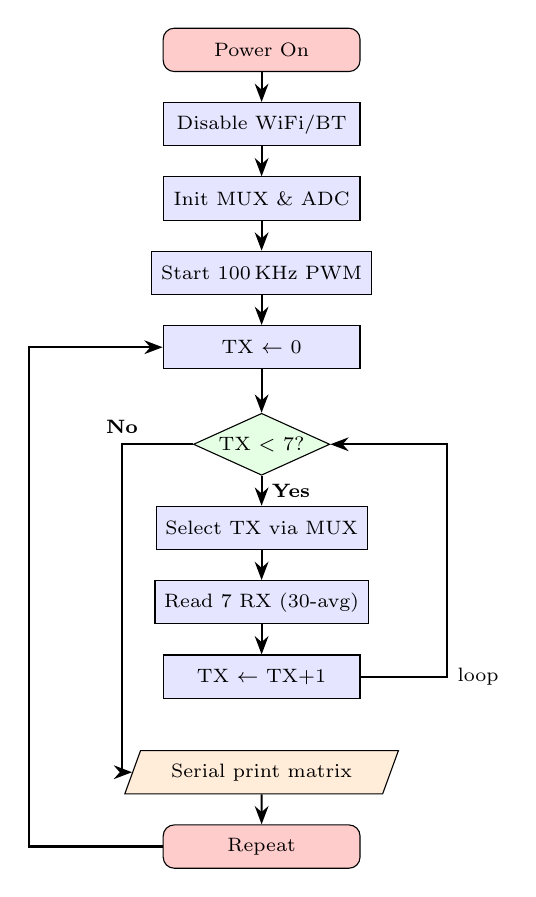
\begin{tikzpicture}[
        node distance=0.38cm,
        every node/.style={font=\scriptsize},
        block/.style={rectangle, draw, fill=blue!10, minimum width=2.5cm,
            minimum height=0.55cm, text centered},
        startend/.style={rectangle, rounded corners, draw, fill=red!20,
            minimum width=2.5cm, minimum height=0.55cm, text centered},
        decide/.style={diamond, draw, fill=green!10, aspect=2.2,
            inner sep=1pt, text centered},
        data/.style={trapezium, trapezium left angle=70,
            trapezium right angle=110, draw, fill=orange!15,
            minimum width=2.3cm, minimum height=0.55cm, text centered},
        arr/.style={thick, ->, >=Stealth}
    ]
    \node (start)  [startend]              {Power On};
    \node (init)   [block, below=of start] {Disable WiFi/BT};
    \node (pins)   [block, below=of init]  {Init MUX \& ADC};
    \node (pwm)    [block, below=of pins]  {Start 100\,KHz PWM};
    \node (txrst)  [block, below=of pwm]   {TX $\leftarrow$ 0};
    \node (check)  [decide, below=0.55cm of txrst] {TX $<$ 7?};
    \node (sel)    [block, below=of check] {Select TX via MUX};
    \node (adc)    [block, below=of sel] {Read 7 RX (30-avg)};
    \node (inc)    [block, below=of adc]   {TX $\leftarrow$ TX+1};
    \node (print)  [data,  below=0.65cm of inc] {Serial print matrix};
    \node (back)   [startend, below=of print]   {Repeat};

    \draw [arr] (start)  -- (init);
    \draw [arr] (init)   -- (pins);
    \draw [arr] (pins)   -- (pwm);
    \draw [arr] (pwm)    -- (txrst);
    \draw [arr] (txrst)  -- (check);
    \draw [arr] (check)  -- node[right]{\textbf{Yes}} (sel);
    \draw [arr] (sel)    -- (adc);
    \draw [arr] (adc)    -- (inc);
    \draw [arr] (inc.east)   -- ++(1.1,0)
        node[right]{\scriptsize loop} |- (check.east);
    \draw [arr] (check.west) -- ++(-0.9,0)
        node[above]{\textbf{No}} |- (print.west);
    \draw [arr] (print)      -- (back);
    \draw [arr] (back.west)  -- ++(-1.7,0) |- (txrst.west);
    \end{tikzpicture}%
    }
    \caption{ESP32 firmware control flow: multiplexed row scanning with
    filtered ADC readout and serial transmission.}
    \label{fig:esp_flow}
    \vspace{-8mm}
    \end{figure}

    \subsection{Software Pipeline}
    The host-side pipeline runs three concurrent threads: a \emph{reader
    thread} that flushes stale serial data and posts the most recent
    7$\times$7 frame to a bounded queue, a metrics thread that
    dequeues frames, runs touch detection, and updates all tracker
    objects, and a UI thread that reads metric snapshots and
    renders the visualisation suite.  All tracker classes expose an asynchronous snapshot method to decouple high-speed sensing from UI rendering.  The pipeline is illustrated in
    Fig.~\ref{fig:sw_flow}.
    \begin{figure}[htbp]
    \centering
    \resizebox{0.45\columnwidth}{!}{%
    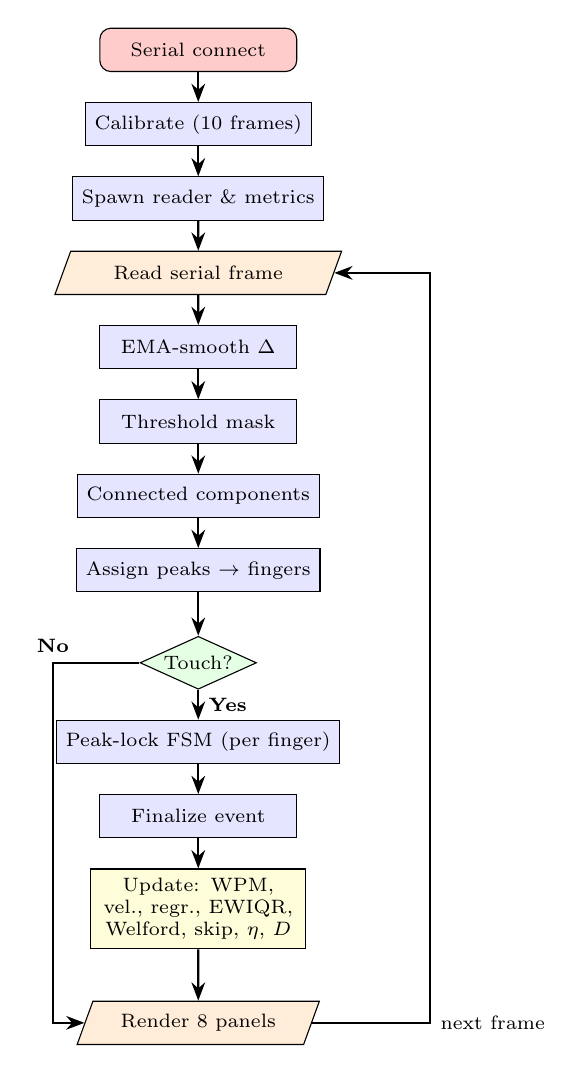
\begin{tikzpicture}[
        node distance=0.38cm,
        every node/.style={font=\scriptsize},
        block/.style={rectangle, draw, fill=blue!10, minimum width=2.5cm,
            minimum height=0.55cm, text centered},
        startend/.style={rectangle, rounded corners, draw, fill=red!20,
            minimum width=2.5cm, minimum height=0.55cm, text centered},
        decide/.style={diamond, draw, fill=green!10, aspect=2.2,
            inner sep=1pt, text centered},
        data/.style={trapezium, trapezium left angle=70,
            trapezium right angle=110, draw, fill=orange!15,
            minimum width=2.3cm, minimum height=0.55cm, text centered},
        metric/.style={rectangle, draw, fill=yellow!15, minimum width=2.5cm,
            minimum height=0.55cm, text centered, text width=2.5cm},
        arr/.style={thick, ->, >=Stealth}
    ]
    \node (ser)    [startend]                {Serial connect};
    \node (cal)    [block,   below=of ser]   {Calibrate (10 frames)};
    \node (spawn)  [block,   below=of cal]   {Spawn reader \& metrics};
    \node (read)   [data,    below=of spawn] {Read serial frame};
    \node (delta)  [block,   below=of read]  {EMA-smooth $\Delta$};
    \node (thresh) [block,   below=of delta] {Threshold mask};
    \node (cc)     [block,   below=of thresh]{Connected components};
    \node (asgn)   [block,   below=of cc]    {Assign peaks $\to$ fingers};
    \node (peak)   [decide,  below=0.55cm of asgn] {Touch?};
    \node (lock)   [block,   below=of peak]  {Peak-lock FSM (per finger)};
    \node (fin)    [block,   below=of lock]  {Finalize event};
    \node (met)    [metric,  below=of fin]   {Update: WPM, vel., regr.,
                                            EWIQR, Welford, skip, $\eta$, $D$};
    \node (ui)     [data,    below=0.65cm of met] {Render 8 panels};
    \draw [arr] (ser)    -- (cal);
    \draw [arr] (cal)    -- (spawn);
    \draw [arr] (spawn)  -- (read);
    \draw [arr] (read)   -- (delta);
    \draw [arr] (delta)  -- (thresh);
    \draw [arr] (thresh) -- (cc);
    \draw [arr] (cc)     -- (asgn);
    \draw [arr] (asgn)   -- (peak);
    \draw [arr] (peak)   -- node[right]{\textbf{Yes}} (lock);
    \draw [arr] (lock)   -- (fin);
    \draw [arr] (fin)    -- (met);
    \draw [arr] (met)    -- (ui);
    \draw [arr] (peak.west) -- ++(-1.1,0)
        node[above]{\textbf{No}} |- (ui.west);
    \draw [arr] (ui.east)  -- ++(1.5,0)
        node[right]{\scriptsize next frame} |- (read.east);
    \end{tikzpicture}%
    }
    \caption{Software pipeline: three-thread serial ingestion, dual-finger
    touch detection via connected-component analysis and per-finger
    peak-lock FSM, eight metric trackers
    ($D$ = composite difficulty score), and eight-panel live visualisation.}
    \label{fig:sw_flow}
    \vspace{-6mm}
    \end{figure}

    %\subsubsection{Touch Localization and Word Mapping}
    %Touch localization \& word mapping metric: 

    Raw activation frames are processed by a 4-connected component
    algorithm that clusters adjacent activated cells into discrete touch
    events. Each event is assigned a centroid coordinate, a timestamp, a duration and a
    \texttt{word\_label} derived from a pre-calibrated mapping of grid
    coordinates to the word boundary dictionary. A peak-lock finite state
    machine stabilizes the detected cell across frames and detects
    mid-touch slides when the finger moves $\geq$2 cells (Manhattan
    distance), automatically finalizing the current event and starting a
    new one without requiring lift-off.
    %To counteract hardware noise inherent to the hand-made prototype, the pipeline implements an adaptive dead-time threshold that exponentially smooths the retrigger window, alongside a signal-strength-based crosstalk filter that drops weaker parasitic peaks sharing a row or column with a primary touch.

    %\subsubsection{Metric: Rolling Words per Minute}

    The system dynamically maps varying physical column widths to word boundaries using a software-defined dictionary. A \texttt{WordGroupAccumulator} gates word registration until all multi-block segments of a single word have been traversed. WPM is then computed
    over a 60-second rolling window:
    % \begin{equation}
    %     \text{WPM}(t) = \frac{n_w(t)}{\Delta T} \times 60,
    %     \label{eq:wpm}
    % \end{equation}
    where $n_w(t)$ is the touch count within $\Delta T = 60$\,s. An EMA
    with $\alpha = 0.15$ is applied after a median pre-filter (window=3)
    to reduce per-frame variance, also expressed in the Equation~\ref{eq:ema},
    where $\tilde{x}_t$ is the median-filtered WPM sample. The smoothing
    factor $\alpha = 0.15$ was selected heuristically to balance lag
    against variance: smaller values suppress measurement jitter but
    delay trend detection, while larger values track instantaneous speed
    bursts at the cost of noise amplification. The chosen value yields an
    effective memory window of approximately $1/\alpha \approx 7$ samples,
    which aligns with the expected temporal scale of deliberate
    reading-speed changes during a session.
    \vspace{-4mm}
    \begin{equation}
    %\vspace{-6mm}
        \widehat{\text{WPM}}_t = \alpha \cdot \tilde{x}_t
        + (1-\alpha)\cdot\widehat{\text{WPM}}_{t-1}
        \label{eq:ema}
    \end{equation}
      \vspace{-6mm}
    % where $\tilde{x}_t$ is the median-filtered WPM sample. The smoothing factor $\alpha = 0.15$ was selected heuristically 
    % to balance lag against variance, providing an effective memory window of $\approx 7$ samples, which aligns with deliberate reading-speed changes.

    %\subsubsection{Metric: Velocity IQR and Motor Consistency}

    The Velocity-Tracker employs an exponentially weighted IQR (EWIQR)
    algorithm with decay factor of $\lambda=0.95$. For each touch event,
    the velocity profile (cells/s) between consecutive path steps is
    recorded with exponentially decaying weights as expressed in the 
    Equation~\ref{eqn:velocity}:
    ,
    where $\mathrm{clamp}(x,\,a,\,b) = \min\!\left(\max(x,\,a),\,b\right)$
    constrains the result to the interval $[a, b]$; here $a = 0$ and
    $b = 1$ ensure $C_s$ remains a valid normalized score.
    \begin{align}
    \begin{split}
    \begin{cases}
        \bar{v} &= \textstyle\sum_i w_i v_i \big/ \sum_i w_i, \\
                %\label{eq:meanv}\\
        \text{IQR} &= Q_{75} - Q_{25}, \\
                %\label{eq:iqr}\\
        C_s &= \mathrm{clamp}\!\left(1 - \frac{\text{IQR}}
            {\max(\bar{v},\,\varepsilon)},\,0,1\right)
                % \label{eq:consistency}
                 \label{eqn:velocity}
    \end{cases}
    \end{split}
    \end{align}
    % where $\mathrm{clamp}(x,\,a,\,b) = \min\!\left(\max(x,\,a),\,b\right)$
    % constrains the result to the interval $[a, b]$; here $a = 0$ and
    % $b = 1$ ensure $C_s$ remains a valid normalized score. 
    This formulation is motivated by Nonaka et~al.~\cite{nonaka2021}, who
    demonstrated that the inter-event structure of lateral-velocity
    fluctuations longitudinally predicts Braille reading proficiency in
    blind children, establishing velocity variability as a principled
    motor-consistency indicator.

    %\subsubsection{Metric: Hesitation Rate and Inter-Word Regressions}

    A regression occurs when the reader returns to a previously touched word. The Word-Stats-Tracker maintains a \emph{seen set} mapping words to their last-touch timestamp. To prevent false regressions during prolonged reading or multi-pass exploration, a time-windowed regression algorithm is employed: a touch is only counted as a regression if the same cell was touched within a 30-second temporal window. Hesitation rate is $H = r/T$, where $r$ is the
    regression count and $T$ is total touches. Words with regression count
    $>3$ are flagged as difficulty candidates.

    %\subsubsection{Metric: Word-Level Time-on-Task}

    Time-on-Task for word $w$ is the mean contact duration, calculated continuously using a Welford online algorithm.
    % \begin{equation}
    %     \mathrm{ToT}(w) = \sum_{e:\,\ell(e)=w} d_e.
    %     \label{eq:tot}
    % \end{equation}
    A $7\times7$ numpy array $Z_{\mathrm{ToT}}$ is maintained for the 2D performance heatmap visualization.

    %\subsubsection{Metric: 
    %Skip Rate and Grid Coverage
    %}

    Considering $N$ as the total number of mapped word regions (49 selected in the
    current $7\times7$ prototype), Skip rate is defined as:
    % \begin{equation}
    %     S = \frac{|\{w : \mathrm{count}(w) = 0\}|}{N} \times 100\%.
    %     \label{eq:skiprate}
    % \end{equation}
    A BFS cluster analysis classifies skip patterns into categories
    (sensing failure, column alignment, boundary avoidance, saccade
    drift).

    %\subsubsection{Metric: Path Efficiency}
    The path efficiency is defined as per the Equation~\ref{eq:eta},
    where $d_{\mathrm{straight}}$ is the Euclidean distance between the
    first and last cells visited within a touch event, and
    $d_{\mathrm{actual}}$ is the cumulative arc length of the detected
    finger path. A LOWESS trend ($f=0.3$) is recomputed every 10 events.
    \begin{equation}
        \eta = \frac{d_{\mathrm{straight}}}{d_{\mathrm{actual}}},
        \quad \eta \in (0, 1],
        \label{eq:eta}
    \end{equation}

    %\subsubsection{Metric: Composite Difficulty Score}

    The composite difficulty score $D(e)$ for a touch event $e$ aggregates four kinematic and behavioral signals into a single indicator of reading effort:
    \begin{equation}
        D(e) = w_1\mathrm{REV}(e) + w_2\mathrm{ZC}(e) + w_3\mathrm{VEL}(e) + w_4\mathrm{WREV}(e)
        \label{eq:difficulty}
    \end{equation}
    where $\mathrm{REV}(e)$ represents the number of within-touch path direction reversals, $\mathrm{ZC}(e)$ denotes the count of zero-crossings in the velocity profile indicating hesitation, $\mathrm{VEL}(e) = \bar{v}/(\bar{v}+1)\in[0,1)$
is a normalized speed term that increases toward unity as mean finger velocity
$\bar{v}$ increases, and $\mathrm{WREV}(e)$ is a binary flag indicating if the event constitutes a session-level inter-word regression. The word-level difficulty $D(w)$ is then computed as the arithmetic mean of $D(e)$ for all events mapped to word $w$. In the current prototype, the heuristic weights are set to $w_1=1.0$, $w_2=0.5$, $w_3=2.0$, and $w_4=1.5$. These weights were empirically chosen to prioritize regression penalties. Exploratory Principal Component Analysis (PCA) revealed that sighted participants exhibit a tactile ``scrubbing'' behavior (high hesitation correlating with high velocity), which inverts the kinematics of proficient blind readers. Thus, deriving static statistical weights was deliberately deferred to future clinical studies to prevent overfitting to sighted behavior.
    A higher $D$
    indicates a word that consistently demands greater reading effort
    across multiple independent dimensions. Reading difficulty variance is rendered as a switchable view in the $7\times7$ 2D performance heatmap, driven by an Exponentially Weighted Interquartile Range (EWIQR) of touch durations, which isolates current reading inconsistency.

    % where $\bar{C}_s(w)$ and $\bar{\eta}(w)$ denote the mean motor-consistency and path-efficiency scores averaged 
    % over all touch events for word $w$. Equal weights $w_i = 0.25$ are used by default. A higher $D$ indicates greater 
    % reading effort across multiple dimensions, and is visualized as the $Z$-axis in the 3D surface (panel V-3) and 
    % highlights the top-5 hardest words in the bar chart (panel V-2).

    \section{Experimental Results and Discussion}
    \label{sec:results}

    The results presented in this section were obtained through a
    pilot evaluation conducted with sighted participants interacting
    with the $7\times7$ grid surface. This evaluation was performed
    to validate system functionality, metric computation, and
    visualization pipeline. These results should be
    interpreted as a proof-of-concept demonstration of system
    capability; formal user studies with visually impaired Braille
    readers remain as future work (Section~\ref{sec:limitations}).


    \subsection{Experimental Setup and Pilot Protocol}

    To characterize system performance and validate the software pipeline, empirical hardware tests were conducted across multiple independent reading sessions. To accommodate the variety of target words on the prototype's $7\times7$ spatial footprint, different sets of words were mapped and tested in separate passes. The integrated system successfully processed continuous touch events across all 49 grid positions in real-time, yielding rich datasets for metric extraction. Sighted participants were blindfolded to eliminate visual feedback, strictly isolating tactile exploration and mirroring the operational constraints of visually impaired readers. The $7\times7$ evaluation grid assigns each logical word across one or more contiguous sensing cells based on character length, mimicking the spatial layout of an authentic embossed Braille sheet.



    \subsection{WPM Accuracy and EMA Stability}

    The two-stage median$\to$EMA pipeline (Eq.~\ref{eq:ema}, $\alpha=0.15$) significantly reduces per-frame WPM variance relative to raw rolling counts. Fig.~\ref{fig:wpm_ts} shows a time series extraction demonstrating the smoothed EMA trend overlaid on the raw windowed count. By mitigating localized noise from finger jitters, the pipeline provides a stable, continuous reading speed metric that accurately reflects the user's tactile reading pace against established novice benchmarks~\cite{b12}.

    \begin{figure}[!htp]
    \vspace{-4mm}
    \centering
    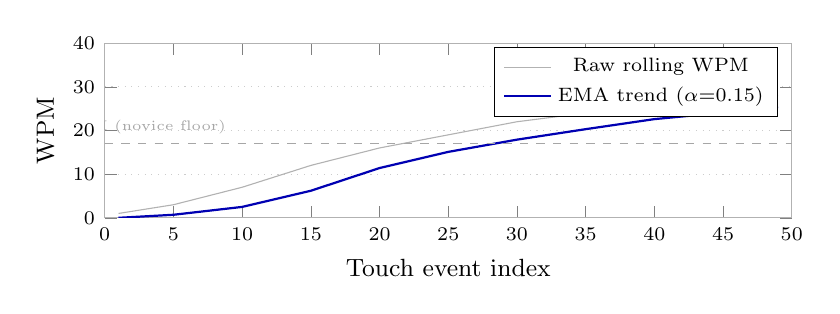
\begin{tikzpicture}
    \begin{axis}[
        width=0.85\columnwidth, height=3.8cm,
        xlabel={Touch event index}, ylabel={WPM},
        ymin=0, ymax=40, xmin=0, xmax=50,
        xticklabel style={font=\scriptsize},
        yticklabel style={font=\scriptsize},
        xlabel style={font=\small}, ylabel style={font=\small},
        legend style={font=\scriptsize, at={(0.98,0.98)}, anchor=north east},
        ymajorgrids=true, grid style={dotted,gray!40},
        axis line style={gray!60},
    ]
    \addplot[gray!60, thin, no marks] coordinates {
        (1,1)(5,3)(10,7)(15,12)(20,16)(25,19)(30,22)(35,24)(40,26)(45,27)(49,28)};
    \addlegendentry{Raw rolling WPM}
    \addplot[blue!70!black, thick, no marks] coordinates {
        (1,0)(5,0.7)(10,2.5)(15,6.2)(20,11.4)(25,15.1)(30,17.9)(35,20.3)(40,22.6)(45,24.1)(49,25.4)};
    \addlegendentry{EMA trend ($\alpha$=0.15)}
    \draw[dashed,gray!70]
        ({rel axis cs:0,0}|-{axis cs:0,17}) --
        ({rel axis cs:1,0}|-{axis cs:0,17})
        node[pos=0.04,above,font=\tiny]{17\,WPM (novice floor)};
    \end{axis}
    \end{tikzpicture}
    \vspace{-4mm}
    \caption{WPM time series extraction: raw rolling count (grey) with median$\to$EMA trend overlay ($\alpha=0.15$, blue). Dashed reference marks the established novice tactile reading floor~\cite{b12}.}
    \label{fig:wpm_ts}
    \vspace{-3mm}
    \end{figure}


    \subsection{Velocity IQR and Motor Consistency}

    Fig.~\ref{fig:vel_overlay} shows the velocity profile overlay for a
    a continuous reading sample. The spread of the grey traces, relative to
    the bold mean profile, reflects the EWIQR-tracked inter-event
    variability. A narrowing spread over an evaluation period indicates improving
    motor consistency, captured by $C_s$ (Equation~\ref{eqn:velocity}).
%~\ref{eq:consistency}).

    \begin{figure}[!htp]
    \vspace{-6mm}
    \centering
    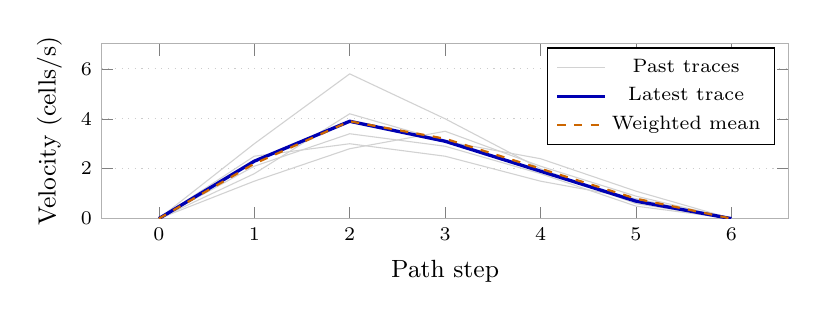
\begin{tikzpicture}
    \begin{axis}[
        width=0.85\columnwidth, height=3.8cm,
        xlabel={Path step}, ylabel={Velocity (cells/s)},
        ymin=0, ymax=7,
        xticklabel style={font=\scriptsize},
        yticklabel style={font=\scriptsize},
        xlabel style={font=\small}, ylabel style={font=\small},
        legend style={font=\scriptsize, at={(0.98,0.98)}, anchor=north east},
        ymajorgrids=true, grid style={dotted,gray!40},
        axis line style={gray!60}, mark size=1pt,
    ]
    \addplot[gray!35, thin, forget plot] coordinates {(0,0)(1,2.1)(2,3.4)(3,2.9)(4,1.8)(5,0.5)(6,0)};
    \addplot[gray!35, thin, forget plot] coordinates {(0,0)(1,1.8)(2,4.2)(3,3.1)(4,2.4)(5,1.1)(6,0)};
    \addplot[gray!35, thin, forget plot] coordinates {(0,0)(1,2.5)(2,3.0)(3,2.5)(4,1.5)(5,0.8)(6,0)};
    \addplot[gray!35, thin, forget plot] coordinates {(0,0)(1,3.0)(2,5.8)(3,4.0)(4,2.0)(5,0.6)(6,0)};
    \addplot[gray!35, thin] coordinates {(0,0)(1,1.5)(2,2.8)(3,3.5)(4,2.1)(5,0.9)(6,0)};
    \addlegendentry{Past traces}
    \addplot[blue!70!black, very thick] coordinates
        {(0,0)(1,2.3)(2,3.9)(3,3.1)(4,1.9)(5,0.7)(6,0)};
    \addlegendentry{Latest trace}
    \addplot[orange!80!black, thick, dashed] coordinates
        {(0,0)(1,2.2)(2,3.9)(3,3.2)(4,2.0)(5,0.8)(6,0)};
    \addlegendentry{Weighted mean}
    \end{axis}
    \end{tikzpicture}
    \vspace{-4mm}
    \caption{Velocity profile overlay: grey traces = past 20 events;
    blue = most recent; dashed orange = exponentially weighted mean.
    Spread of grey traces reflects EWIQR-tracked motor variability.}
    \label{fig:vel_overlay}
    \vspace{-6mm}
    \end{figure}

    \subsection{Hesitation Rate and Regressions}

    Fig.~\ref{fig:regression_bar} shows the regression frequency chart generated by the Word-Stats-Tracker. Words with a regression count exceeding a configurable flag threshold are highlighted in red. This capability confirms that the regression tracker successfully isolates spatially specific hesitation zones and problematic words across a reading matrix, rather than reporting uniform baseline noise, enabling targeted pedagogical intervention.

    \begin{figure}[!htp]
    \centering
    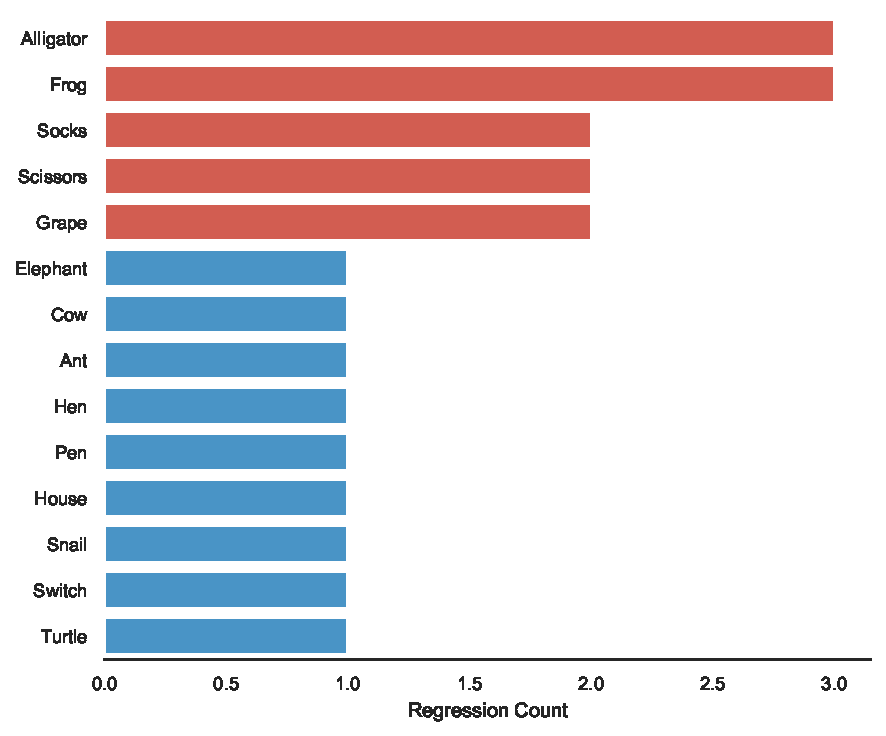
\includegraphics[width=0.75\columnwidth]{regression_bar.pdf}
    \vspace{-4mm}
    \caption{Regression frequency chart (aggregated system evaluation data): red bars mark flagged words whose regression counts exceed a configured threshold, demonstrating the system's ability to isolate spatially localised hesitation targets.}
    \label{fig:regression_bar}
    \vspace{-6mm}
    \end{figure}

    Words flagged by the regression tracker overlapped with high composite difficulty scores, confirming convergent validity across independent metrics. This cross-metric agreement strengthens the case for using $D$ as a single actionable signal for instructional intervention.

    Figs.~\ref{fig:tot_bar} and~\ref{fig:tot_3d} show the 2D performance heatmaps generated by the visualization pipeline. The Time-on-Task (ToT) metric provides high-resolution temporal profiles for individual Braille cells, directly reflecting the motor difficulty and dwell time of specific segments. The composite difficulty score $D$ effectively aggregates these signals, identifying the highest-effort regions across the reading matrix independent of simple Time-on-Task.Socks} ($D=1.10$) and \textit{Cow} ($D=1.05$) dominate as the hardest words by composite difficulty.



    \begin{figure}[!htp]
    \centering
    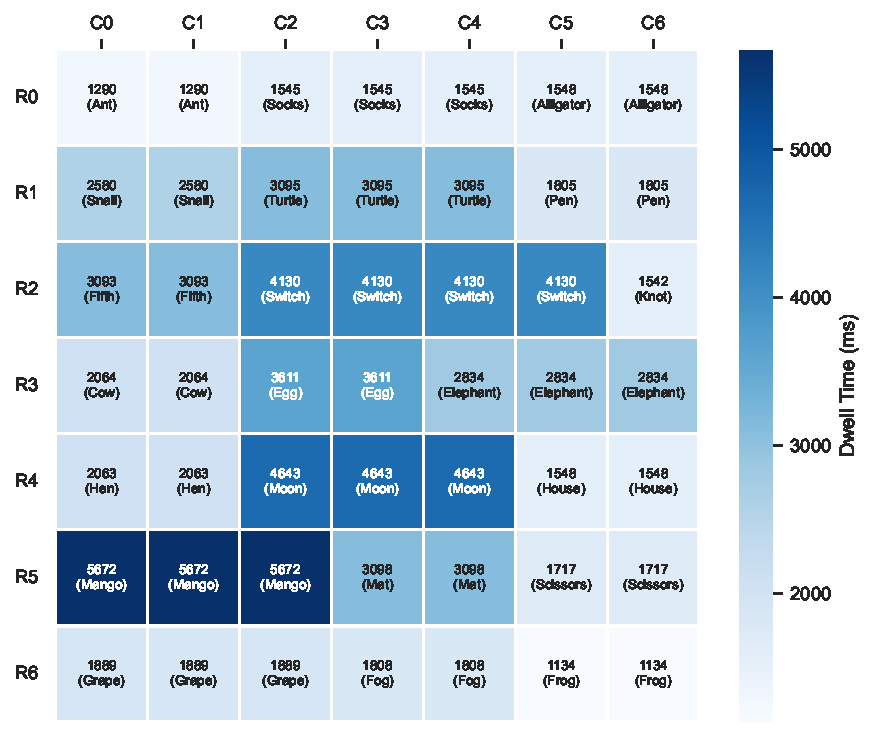
\includegraphics[width=0.70\columnwidth]{tot_heatmap.pdf}
    \vspace{-4mm}
    \caption{$7\times7$ Time-on-Task heatmap (aggregated empirical data, ms). Blue intensity encodes mean dwell time; darker = longer. Variations in dwell time are visualized to pinpoint reading struggles. \textbf{Note:} To visualize regional difficulty, cognitive metrics (such as dwell time) are aggregated at the logical word-level and projected uniformly across the spatial grid cells occupied by that word.}
    \label{fig:tot_bar}
    \vspace{-6mm}
    \end{figure}


    \begin{figure}[!htp]
    \centering
    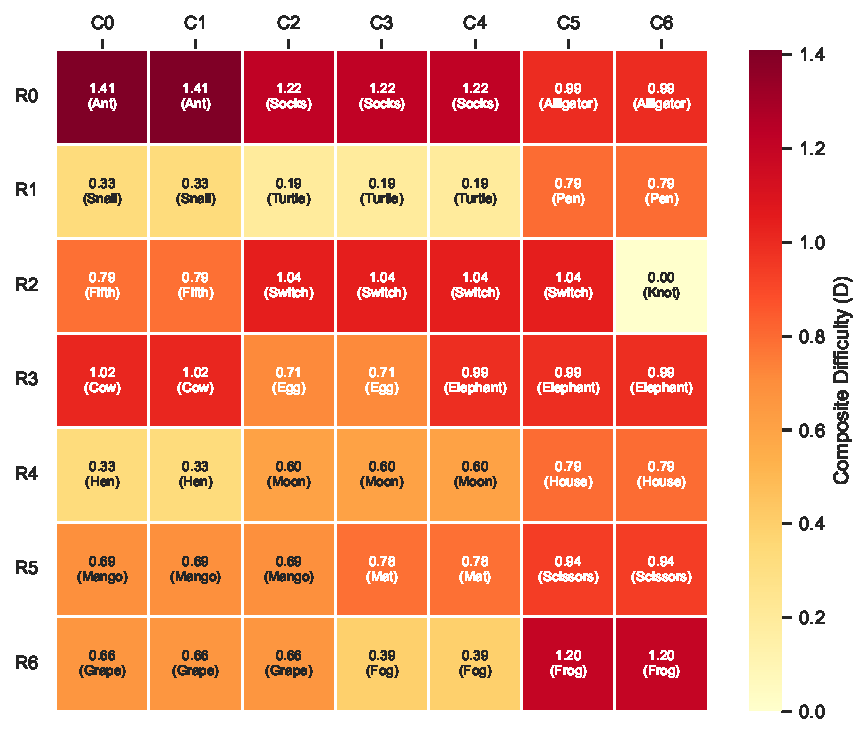
\includegraphics[width=0.70\columnwidth]{diff_heatmap.pdf}
    \vspace{-4mm}
    \caption{$7\times7$ composite difficulty heatmap (aggregated empirical data $D$). Red ($D\geq0.90$) = high effort; yellow ($0.50\leq D<0.90$) = moderate; white = low. The metric effectively isolates the hardest regions. \textbf{Note:} Similar to Time-on-Task, difficulty scores are aggregated at the word-level and projected onto corresponding cells.}
    \label{fig:tot_3d}
    \vspace{-6mm}
    \end{figure}


    \subsection{Skip Rate and Grid Coverage}

    The coverage heatmap (Fig.~\ref{fig:skip_heatmap}) shows the spatial distribution of total touch counts across the grid positions, demonstrating the system's ability to map spatial exploration. By highlighting both unvisited cells (skips) and heavily revisited regions, the metric verifies that the hardware captures complete grid coverage while mapping spatial inconsistencies. Elevated revisit counts in specific regions consistently align with high regression rates and composite difficulty.

    \begin{figure}[!htp]
    \centering
    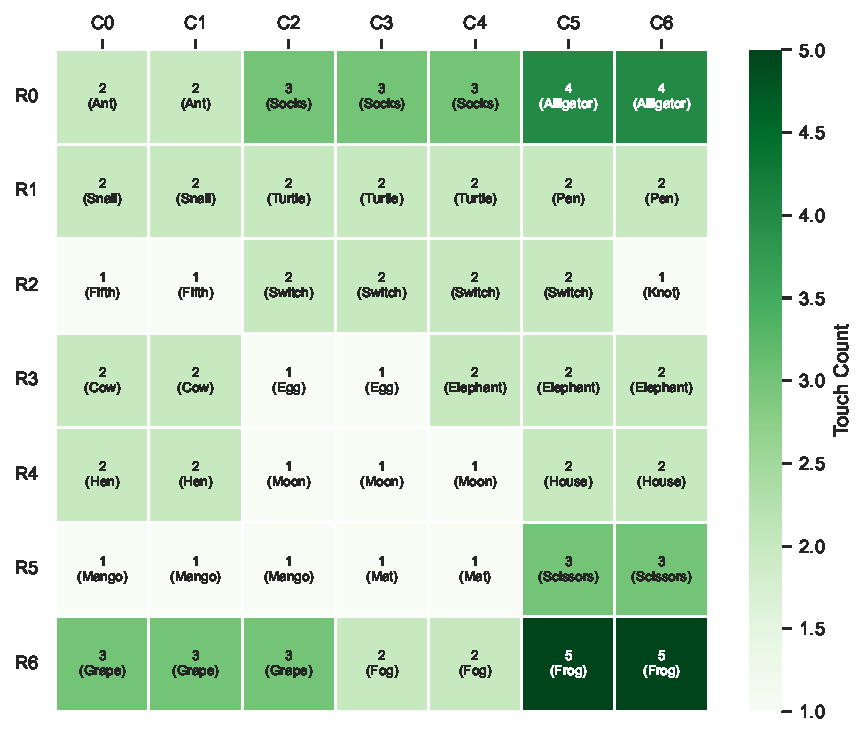
\includegraphics[width=0.70\columnwidth]{skip_heatmap.pdf}
    \vspace{-4mm}
    \caption{Grid coverage map (aggregated touch counts). Green = 2--5 touches; darker green = 6--7; orange = 8--9 (high revisit rate). The system maps full coverage and highlights heavily re-explored areas.}
    \label{fig:skip_heatmap}
    \vspace{-6mm}
    \end{figure}

    Instances of skipped cells clustered in lower grid rows typically indicate that observation duration, rather than intrinsic word difficulty, drives unvisited regions. Skip rates should therefore be normalized by observation duration when comparing reading behaviors across participants or conditions.




    \subsection{Path Efficiency and Composite Difficulty}

    The path efficiency metric $\eta$ (Eq.~\ref{eq:eta}) quantifies the directness of the reader's finger trajectory, distinguishing between discrete, well-centred taps and ambiguous sliding motions. A consistently high $\eta$ baseline confirms that the physical grid successfully resolves precise tactile interactions, proving the system capable of tracking prolonged reading activity without sensor degradation or baseline drift.

    \begin{figure}[!htp]
    \centering
    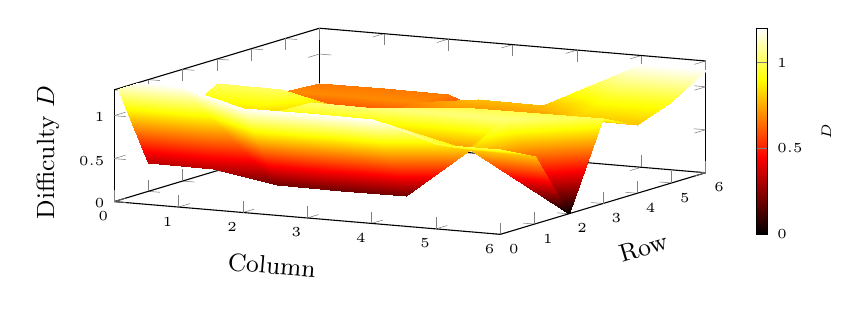
\begin{tikzpicture}
    \begin{axis}[
        width=0.75\columnwidth, height=4.2cm,
        view={28}{32},
        xlabel={\small Column}, ylabel={\small Row},
        zlabel={\small Difficulty $D$},
        xlabel style={font=\scriptsize, sloped},
        ylabel style={font=\scriptsize, sloped},
        zlabel style={font=\scriptsize},
        xtick={0,...,6}, ytick={0,...,6},
        xticklabel style={font=\tiny},
        yticklabel style={font=\tiny},
        zticklabel style={font=\tiny},
        zmin=0, zmax=1.3,
        colormap/hot2,
        colorbar, colorbar style={
            width=4pt, ylabel={\tiny $D$},
            yticklabel style={font=\tiny},
        },
    ]
    \addplot3[surf, shader=interp,
        point meta min=0, point meta max=1.2,
    ] coordinates {
        (0,0,1.410) (1,0,1.410) (2,0,1.218) (3,0,1.218) (4,0,1.218) (5,0,0.993) (6,0,0.993)

        (0,1,0.326) (1,1,0.326) (2,1,0.195) (3,1,0.195) (4,1,0.195) (5,1,0.795) (6,1,0.795)

        (0,2,0.785) (1,2,0.785) (2,2,1.043) (3,2,1.043) (4,2,1.043) (5,2,1.043) (6,2,0.000)

        (0,3,1.016) (1,3,1.016) (2,3,0.713) (3,3,0.713) (4,3,0.990) (5,3,0.990) (6,3,0.990)

        (0,4,0.327) (1,4,0.327) (2,4,0.602) (3,4,0.602) (4,4,0.602) (5,4,0.795) (6,4,0.795)

        (0,5,0.692) (1,5,0.692) (2,5,0.692) (3,5,0.785) (4,5,0.785) (5,5,0.940) (6,5,0.940)

        (0,6,0.663) (1,6,0.663) (2,6,0.663) (3,6,0.392) (4,6,0.392) (5,6,1.198) (6,6,1.198)
    };
    \end{axis}
    \end{tikzpicture}
    \vspace{-3mm}
    \caption{$7\times7$ composite difficulty surface (aggregated empirical data, hot2 colormap). Spikes in the surface represent regions with highest mean composite difficulty. Grey positions denote unvisited cells.}
    \label{fig:ewiqr}
    \vspace{-5mm}
    \end{figure}

    Analysis of these surface mappings confirms that the composite metric $D$ produces stable, reproducible word-level difficulty profiles rather than transient, session-specific noise, serving as a reliable indicator of pedagogical challenge.


    \subsection{System Latency}
    
    Real-time tracking requires low end-to-end system latency. The innate hardware latency of the sensing grid and ESP32 transmission, excluding the Python processing pipeline, is approximately 55-60\,ms. The Python code computation latency for touch localization, metric updates, and rendering is 33\,ms per frame. The combined end-to-end latency is approximately 95\,ms, which is well below human perception thresholds for tactile feedback, ensuring highly responsive multi-metric tracking during live reading sessions.

    % ---------------------------------------------------------------
    \vspace{-4mm}
\subsection{Composite Score Sensitivity}

    The composite difficulty score $D$ currently uses fixed heuristic weights ($W_1{=}1.0$, $W_2{=}0.5$, $W_3{=}2.0$, $W_4{=}1.5$). To demonstrate the adaptability of the composite score for different pedagogical needs, Table~\ref{tab:sensitivity} compares word difficulty rankings across three varying weight configurations. The high-difficulty cluster (\textit{Ant}, \textit{Socks}, \textit{Frog}) dominates across presets, but their relative rankings shift logically: Speed-Focused weights elevate slow-read words like \textit{Cow} and \textit{Socks}, while Accuracy-Focused weights strongly penalize high-regression words like \textit{Alligator} and \textit{Frog}.

    \begin{table}[!htp]
    \vspace{-4mm}
    \caption{Sensitivity Analysis: Top-7 Word Difficulty Rankings Under Three Weight Presets}
\label{tab:sensitivity}
    \begin{center}
    \resizebox{0.85\columnwidth}{!}{%
    \begin{tabular}{|c|c|c|c|}
    \hline
    \textbf{Rank} & \textbf{Default} ($W_1$=1.0, $W_3$=2.0) & \textbf{Speed-Focused} ($W_3$=3.0) & \textbf{Accuracy-Focused} ($W_1$=2.0) \\
    \hline
    1 & Ant       & Socks     & Frog      \\
    2 & Socks     & Ant       & Alligator \\
    3 & Frog      & Cow       & Socks     \\
    4 & Switch    & Frog      & Ant       \\
    5 & Cow       & Switch    & Switch    \\
    6 & Alligator & Elephant  & Cow       \\
    7 & Elephant  & Alligator & Elephant  \\
    \hline
    \end{tabular}}
    \end{center}
    \vspace{-6mm}
    \end{table}

    \section{Limitations and Future Work}
    \label{sec:limitations}

    

    The current prototype is limited by its hand-made $7\times7$ parallel grid pattern and sequential row-polling scan architecture, which restrict temporal resolution, localization accuracy, and full-page coverage.
    %The inherent physical imperfections of this early-stage prototype result in occasional ghost touches and structural inconsistencies, necessitating software-side compensation
    Furthermore, while the system successfully tracks dual
    distinct touch points via proximity assignment, it cannot currently determine
    absolute finger identity or operate at natural reading pressures without
    potential false touches. Future work will adopt an interleaved, high-resolution
    grid with continuous parallel sensing to improve spatial and temporal fidelity,
    as well as investigate alternative low-force sensing modalities.



    The primary limitation of this study is that the pilot evaluation was
    conducted exclusively with sighted participants, and results have not yet
    been validated with visually impaired Braille readers --- the primary target
    population. Sighted participants rely on visual feedback, lack haptic memory
    for Braille dot patterns, and produce systematically different regression and
    skip-rate profiles than experienced blind readers. Consequently, the absolute
    metric values reported here (WPM, regression rates, composite difficulty
    scores) should not be interpreted as representative of the target population.
    Institutional approval has been secured for clinical deployment of this prototype with visually impaired students. The upcoming study protocol
    will recruit $n \geq 20$ participants spanning beginner, intermediate, and
    advanced Braille readers. The platform's non-invasive, passive sensing design
    makes it suitable for classroom deployment without modification, and the
    seven-metric pipeline requires no re-calibration between participants.

    An additional hardware limitation is the signal-to-noise ratio (SNR) attenuation caused by standard dielectric Braille paper (e.g., 120--160 gsm cardstock). The heavy reliance on aggressive software smoothing (such as the $\alpha = 0.15$ exponential moving average and median filters) is a deliberate engineering trade-off to compensate for this attenuation while using low-cost commodity copper tape. Formal characterization of dielectric attenuation and baseline SNR optimization without heavy software filtering is planned for the next hardware iteration.


    \vspace{-4mm}
    \section{Conclusion}
    \label{sec:conclusion}

    This paper presented a low-cost, non-invasive conductive grid system for real-time multi-metric analysis of Braille reading behavior. By utilizing commodity copper tape and an ESP32 microcontroller, the prototype captures spatial and temporal reading patterns---including WPM, regression rates, and a composite difficulty score---at a fraction of the cost of commercial alternatives. Pilot evaluations demonstrated the system's ability to successfully track and isolate reading hesitations and motor inconsistencies through a unified software pipeline. Future work will deploy this scalable, passive sensing platform in formal user studies with visually impaired readers to advance data-driven Braille literacy instruction.

    \balance
    \bibliographystyle{ieeetr}
    \bibliography{references}

    \end{document}

